\section{Description}
Assume you are the project manager for a software development project. 
You want to have a dashboard to see how things are going.\newline\newline
\noindent
Assuming the following in-process metric data, create a Trouble Report 
Arrival Plan:
\begin{enumerate}
    \item Total size of the sofware: \textbf{10 KLOC}
    \item TR arrival to be algorithmically: \textbf{10\%, 80\%, 10\% per week after each weekly turnover}
    \item Defect Density: \textbf{10 defects per KLOC before you ship}
\end{enumerate}

\begin{figure}[!htb]
    \centering
    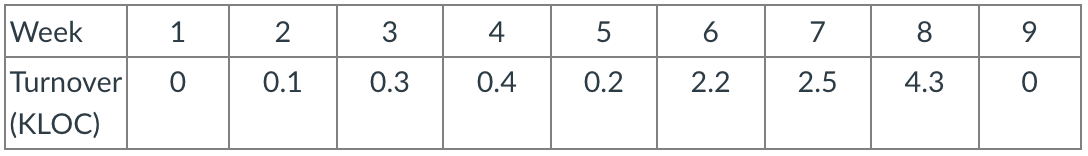
\includegraphics[scale=0.57]{integration-plan.png}    
    \caption{Integration Plan}
\end{figure}

\pagebreak

\section{Defects Arrival}
The first thing we need to do is calculate how many defects are we going 
to receive, according to the description we are receiving 10 defects 
per KLOC. \newline\newline
\noindent
So we are going to multiple the turnover of each week by 10 to learn how many defects are
we receiving each week.

\begin{figure}[!htb]
    \centering
    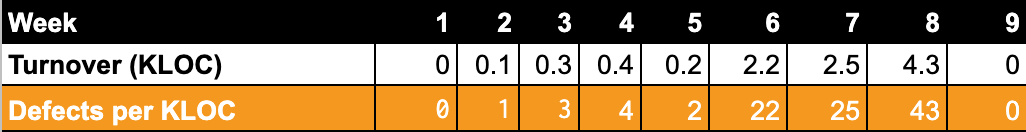
\includegraphics[scale=0.57]{defects-per-kloc.png}    
    \caption{Defects per KLOC}
\end{figure}
\noindent
Now that we know how many defects we are receiving we need to calculate how they 
will arrive, we know that 10\% of them are coming in the first week from ship, 
80\% is coming the following week and the remaining 10\% is coming in the third 
week after the code was turnover.

\begin{figure}[!htb]
    \centering
    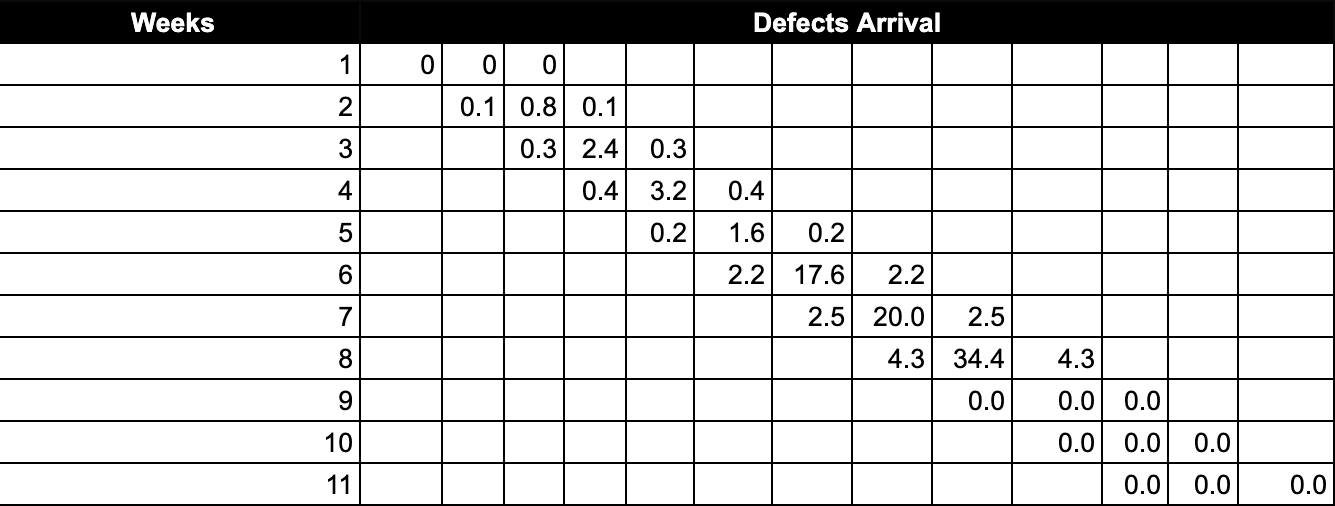
\includegraphics[scale=0.57]{defect-arrival-calculation.png}    
    \caption{Defects arrival calculation}
\end{figure}
\noindent
In Figure 3 we go through each week and we split the value of the defects 
that we receive that week and split them across 3 weeks, in the first week we do 
not receive any code so we have 0 defects, but starting from week 2 we start 
receiving defects that are spread in three weeks.

\pagebreak

\begin{figure}[!htb]
    \centering
    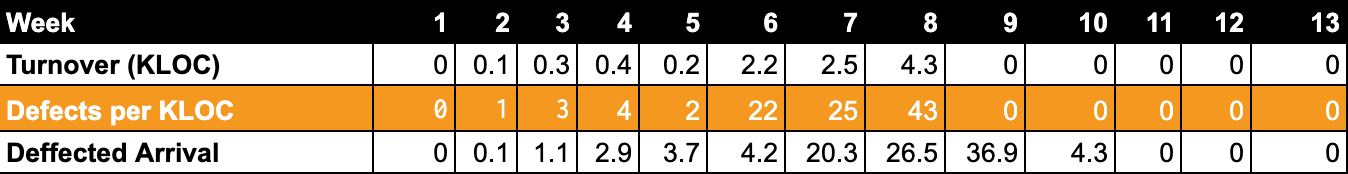
\includegraphics[scale=0.57]{defect-arrival.png}    
    \caption{Defects arrival per week}
\end{figure}
\noindent
We have the spread of all the defects, but you not only get the defects from 
that week, you still get the defects from the previous week, using the values 
from Figure 3, we sum all the defects from each week and the result is 
shown in Figure 4. With this information, we are ready to create a backlog 
plan.